\chapter{Processes}

\section{Threads}

\subsection{Threads vs. processes}

\begin{tabular}{p{7cm} p{7cm}}
\textbf{processes}			&\textbf{threads}\\
-execution of program			&-several threads share CPU\\
-processor creates virtual processor	&-thread context has little memory information, perhaps mutex lock\\
-for each program everyting is stored in process table	&-threads avoid blocking application (e.g. spreadsheet,computation of dependent cells, intermediate backup)\\
-transparent sharing of resources,(processor, memory) separation&-thread switch is fast\\
-each virtual processor has it's own independent adress space & \ \\
-process switch is expensive, (save cpu context, pointers, translation lookaside buffer (TLB), memory management unit (MMU)) & \ \\
-perhaps even swaps to disk, if memory exhausted & \ \\
\end{tabular}

\ \\

\textbf{Summary:}
\begin{compactitem}
	\item Serveral threads share one process.
	\item Processes have own address space, threads don't.
	\item Processes and threads each have userland and kernel implementations
\end{compactitem}

\subsection{Thread implementation}

\begin{compactitem}
	\item \textbf{thread package} operations to create and destroy threads, operations for synchronization (mutexes / condition variables)
	\item user-level thread library
	\begin{compactitem}
		\item it is cheap to create and destroy threads
		\item switching thread context can often be done in just a few instructions
		\item invocation of a blocking system call will immediately block the entire process to which the thread belongs, and thus also all the other threads in that process
	\end{compactitem}
	\item threads implemented in kernel-space	
	\begin{compactitem}
		\item circumvents the blocking problem
		\item thread operations need system calls
		\item switching thread contexts may now become as expensive as switching process contexts
		\item most of the performance benefits of using threads instead of processes then disappears
	\end{compactitem}
\end{compactitem}

\subsubsection{Two approaches to combine the advantages of user- and kernel space thread packages}
\begin{compactenum}
	\item \textbf{Light-weight processes}
	\begin{compactitem}
		\item hybrid form of user-level and kernel-level threads
		\item LWP runs in the context of a single (heavy-weight) process, and there can be several LWPs per process
		\item offers a user-level thread package \\ 
		$\Rightarrow$ all operations on threads are carried out without intervention of the kernel
		\item thread package has a single routine to schedule the next thread
		\item when an LWP finds a runnable thread, it switches context to that thread.
		\item other LWPs may be looking for other runnable threads as well
		\item thread may block on system call, then other LWP may run
		\item Advantages of LWP and user-level thread package
		\begin{compactitem}
			\item creation, deletion etc is easy, no kernel intervention
			\item blocking syscall does not suspend process if enough LWPs are available
			\item applications do not see LWP. They only see user-level threads
			\item LWP can run on different processors in multiprocessor systems
		\end{compactitem}
		\item Disadvantage: LWP creation as expensive as creation of kernel-level thread \\
	\end{compactitem}
	\item \textbf{Scheduler activation} upcall to achieve process switch
	\begin{compactitem}
		\item most essential difference between scheduler activations and LWPs is that when a thread blocks on a system call, the kernel does an upcall to the thread package, effectively calling the scheduler routine to select the next runnable thread
		\item advantage: saves management of LWPs by the kernel
		\item use of upcalls is considered less elegant, as it violates the structure of layered systems, in which calls only to the next lower-level layer are permitted
	\end{compactitem}	
\end{compactenum}

\begin{figure}[h]
	\centering
	\includegraphics[width=300px]{gfx/lwps.png}
	\caption{Combining kernel-level lightweight processes and user-level threads}
	\label{img:lwps}
\end{figure}

\subsection{Threads in Distributed Systems}

\subsubsection{Multithreaded Clients}

\begin{compactitem}
	\item multiple thread may hide communication delay (distribution transparency)
	\item web browser opens several connections to load parts of a document/page
	\item web server may be replicated in same or different location\\
	$\Rightarrow$ truly parallel access to items and parallel download
\end{compactitem}

\subsubsection{Multithreaded Server}

\begin{compactitem}
	\item single threaded, e.g. file server
	\begin{compactitem}
		\item thread serves incoming request, waits for disk, returns file
		\item serves next
	\end{compactitem}
	\item multithreaded
	\begin{compactitem}
		\item dispatcher thread recieves request
		\item hands over to worker thread
		\item waits for disk etc.
		\item dispatcher takes next request
	\end{compactitem}
	\item finite state machine
	\begin{compactitem}
		\item only one thread
		\item examines request, either read from cache (do delay) or from disk (send message to disk, store request) 
		\item requests waiting for answer are stored in table (state)
		\item while waiting for answers, e.g. from disk, serves next request
		\item next message may either be a request for new work or a reply from the disk about a previous operation
		\item if reply from disk, fetch info from table and reply to client
		\item In effect, we are simulating threads and their stacks
		\item process acts as finite state machine that receives messages and acts/changes state
	\end{compactitem}		
\end{compactitem}
\ \\
\ \\
\begin{tabular}{l | l}
\textbf{model} 		&	\textbf{characteristics} \\ \hline
single thread 		& 	no parallelism, blocking syscalls \\
multithreaded 		&	parallelism, blocking syscalls \\
finite state machine 	&	parallelism, needs non-blocking syscalls \\
\end{tabular}

\section{Virtualization}

\begin{figure}[h]
	\centering
	\includegraphics[width=350px]{gfx/virtualization_1.png}
	\caption{ (a) General organization between a program, interface, and system. 
			 (b) General organization of virtualizing system A on top of system B.}
	\label{img:virtualization_1}
\end{figure}

\begin{compactitem}
	\item (resource) virtualization pretends there are more resources then available
	\item application software is mostly always outliving its underlying systems software and hardware \\
	$\Rightarrow$ need for virtualization
\end{compactitem}


\subsection{The Role of Virtualization in Distributed Systems}

\begin{compactitem}
	\item virtualization deals with extending or replacing an existing interface so as to mimic the behavior of another system
	\item networking has become pervasive
	\begin{compactitem}
		\item heterogeneous hardware environment
		\item reduce diversity by letting applications run on its own virtual machine (possibly including libraries and OS)\\
		$\Rightarrow$ improves portability
	\end{compactitem}
\end{compactitem}


\subsection{Architectures of Virtual Machines}

\begin{figure}[h]
	\centering
	\includegraphics[width=350px]{gfx/virtualization_2.png}
	\caption{ (a) A process virtual machine, with multiple instances of (application, runtime) combinations. 
			 (b) A virtual machine monitor. with multiple instances of (applications, operating system) combinations}
	\label{img:virtualization_2}
\end{figure}

\begin{compactenum}	
	\item \textbf{Process Virtual Machine}	
	\begin{compactitem}
		\item provides an abstract instruction set that is to be used for executing applications
		\item instructions can be interpreted (as is the case for the Java runtime environment) or
		\item instructions can be emulated (e.g. Wine for running Windows applications on UNIX machines)
	\end{compactitem}
	
	\item \textbf{Virtual machine monitor}	
	\begin{compactitem}
		\item provide a system that is as a layer completely shielding the original hardware
		\item offering the complete instruction set of that same (or other hardware) as an interface
		\item this interface can be offered simultaneously to different programs\\
		$\Rightarrow$ run multiple and possibly different operating systems concurrently on the same platform
		\item Examples: VMware, Xen		
	\end{compactitem}
\end{compactenum}


\section{Clients}

A closer look of the clients (in the client-server model).

\begin{minipage}{\linewidth}
      \centering
      \begin{minipage}{0.47\linewidth}
          \begin{figure}[H]
	           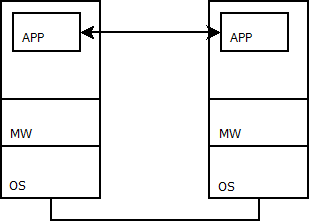
\includegraphics[width=180px]{gfx/clienta.png}
               \caption{a) app specific communication}
          \end{figure}
      \end{minipage}
      \hspace{0.05\linewidth}
      \begin{minipage}{0.47\linewidth}
          \begin{figure}[H]
        	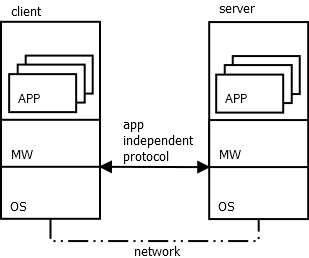
\includegraphics[width=180px]{gfx/clientb.png}
            \caption{b) machine only communication}
            	\label{img:application_independent_proto}
          \end{figure}
      \end{minipage}
\end{minipage}
\ \\

\subsection{Different kinds of Clients}

\begin{compactenum}
	\item \textbf{Networked Application}
	\begin{compactitem}
		\item remote service has a separate counterpart on the client machine that communicates with the server
		\item an application-level protocol will handle the synchronization
		\item Example: agenda running on a user's PDA that needs to synchronize with a remote, possibly shared agenda
	\end{compactitem}
	\item \textbf{Networked User Interface / Thin Client}
	\begin{compactitem}
		\item provide direct access to remote services by only offering a convenient user interface
		\item client machine is used only as a terminal with no need for local storage (thin client)
		\item application-neutral communication protocol solution (see \ref{img:application_independent_proto})
		\item thin client approach only works with good separation of application logic from user interaction
		\item \textbf{Example: X-Windows}
		\begin{compactitem}
			\item example for thin client
			\item bad separation between application logic and user interaction \\
			$\Rightarrow$ lot of synchronous communication $\Rightarrow$ bad performance
			\item compression of interaction commands can alleviate problem
		\end{compactitem}
		\item \textbf{Compound Documents}
		\begin{compactitem}
			\item a collection of documents, possibly of very different kinds (like text, images, spreadsheets, etc.
			\item seamlessly integrated at the user-interface level
			\item he applications associated with a compound document do not have to execute on the client's machine
		\end{compactitem}		
	\end{compactitem}
\end{compactenum}

\section{Servers}


\begin{compactitem}
	\item server is a process implementing a specific service on behalf of a collection of clients
	\item it waits for an incoming request from a client 
	\item ensures that the request is taken care of
	\item waits for the next incoming request
\end{compactitem}

\subsection{Kinds of server}

\begin{compactdesc}
	\item[Iterative Server] \ 
	\begin{compactitem}
		\item server itself handles the request and, if necessary, returns a response to the client
	\end{compactitem}
	\item[Concurrent Server] \  
	\begin{compactitem}
		\item does not handle the request itself, but passes it to a separate thread or another process
		\item after which it immediately waits for the next incoming request
		\item Example 1: multithreaded server 
		\item Example 2: fork a new process for each new incoming request ($\rightarrow$ UNIX)
	\end{compactitem}
\end{compactdesc}

\subsection{Communication Endpoints}

\begin{compactitem}
	\item clients send re- quests to an end point (port), at the machine where the server is running
	\item each server listens to a specific end point. 
	\item how do clients know the end point of a service?
\end{compactitem}

\subsubsection{Fixed Preassigned Endpoints}
\begin{compactitem}
	\item globally assign end points for well-known services
	\item Example: HTTP server always listens to TCP port 80
	\item server listens to port, endpoint to the client; some ports are reserved for special services
	\item stateless servers, keeps no information on state of client $\rightarrow$ change state without informing the client, e.g. web server
\end{compactitem}

\subsubsection{Dynamically Assigned Endpoints: Daemons}

\begin{compactitem}
	\item service gets dynamically assigned port
	\item client needs to look up the endpoint first
	\item daemon with well known endpoint keeps track of all running services
	\item daemon delivers endpoint to client
\end{compactitem}

\subsubsection{Dynamically Assigned Endpoints: Superserver}

\begin{compactitem}
	\item a single superserver listening to each end point associated with a specific service
	\item when a request comes in, the daemon forks a process to take further care of the request
	\item 
\end{compactitem}

\begin{minipage}{\linewidth}
      \centering
      \begin{minipage}{0.45\linewidth}
          \begin{figure}[H]
	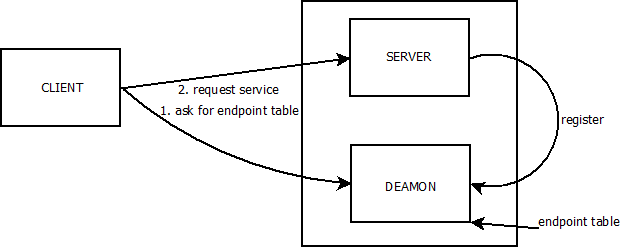
\includegraphics[width=200px]{gfx/server_deamon.png}
	\caption{listener server}
	\label{img:listener}
          \end{figure}
      \end{minipage}
      \hspace{0.05\linewidth}
      \begin{minipage}{0.45\linewidth}
          \begin{figure}[H]
	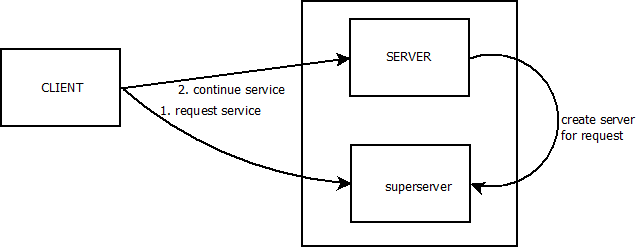
\includegraphics[width=200px]{gfx/superserver.png}
	\caption{superserver}
	\label{img:supserv}
          \end{figure}
      \end{minipage}
\end{minipage}

\subsection{State}

\subsubsection{Stateless Server}

\begin{compactitem}
	\item does not keep information on the state of its clients
	\item can change its own state without having to inform any client
	\item Example: Webserver
	\begin{compactitem}
		\item responds to incoming HTTP requests
		\item when the request has been processed, the Web server forgets the client completely
	\end{compactitem}
	\item the server may maintain information on its clients, but if this information is lost, it will not lead to a disruption of the service offered
	\item cookies allow to share information for server upon next visit client sends it's cookies \\
	$\Rightarrow$ allows state information for stateless server
\end{compactitem}

\subsubsection{Softstate Server}

\begin{compactitem}
	\item a particular form of a stateless design
	\item the server promises to maintain state on behalf of the client, but only for a limited time
	\item when time has expired, all information on client is discarded
	\item Example: a server promising to keep a client informed about updates, but only for a limited time
\end{compactitem}

\subsubsection{Stateful server}

\begin{compactitem}
	\item maintains persistent information on its clients
	\item the information needs to be explicitly deleted by the server
	\item Example: Fileserver with update operations
	\begin{compactitem}
		\item allows client to keep copy of a file and perform update operations
		\item server maintains a table with \emph{(client, file)} associations
		\item table allows server to keep track of which client currently has the update permissions on which file
	\end{compactitem}
	\item stateful servers often offer performance gains compared to stateless designs 
	\item higher complexity, especially in cases of crashes (need for recovery)
\end{compactitem}

\begin{minipage}{\linewidth}
      \centering
      \begin{minipage}{0.45\linewidth}
          \begin{figure}[H]
	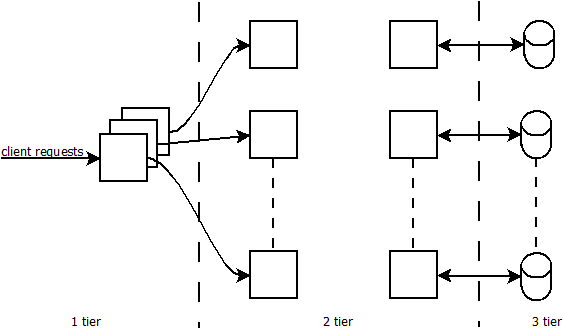
\includegraphics[width=180px]{gfx/server3.png}
	\caption{stateless server}
	\label{img:statel_serv}
          \end{figure}
      \end{minipage}
      \vline
      \hspace{0.05\linewidth}
      \begin{minipage}{0.45\linewidth}
          \begin{figure}[H]
	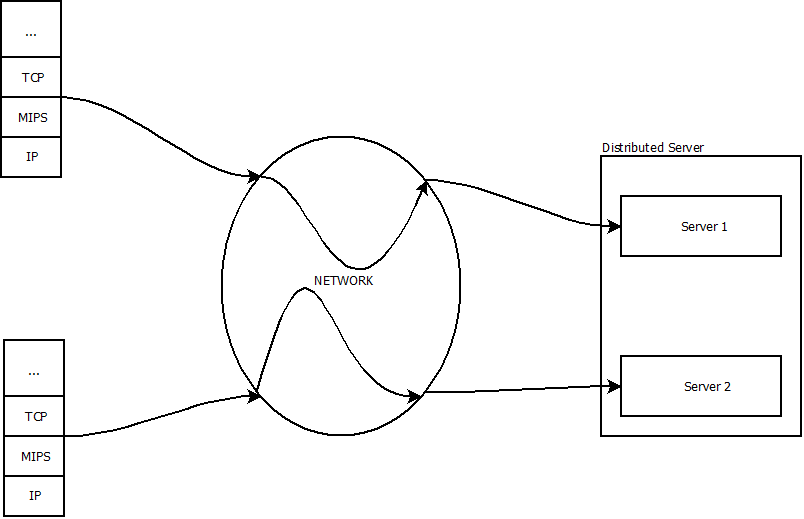
\includegraphics[width=180px]{gfx/distrb_server.png}
	\caption{distributed server}
	\label{img:distrb_serv}
          \end{figure}
      \end{minipage}
\end{minipage}

\subsection{Distributed Servers}

\begin{compactitem}
	\item a possibly dynamically changing set of machines, with also possibly varying access points, but which nevertheless appears to the outside world as a single machine
	\item how to manage the endpoints of the different machines?
	\begin{compactenum}
		\item DNS: servers in different locations with different IPs can have the same name in DNS
		\item MIPv6: mobility support for IPv6
		\begin{compactitem}
			\item mobile node has home network with stable home adress (HoA)
			\item special router is home agent and takes care of traffic to the mobile node
			\item mobile node receives care-of-adress (CoA), never seen by client
			\item route optimisation avoids routing through home agent		
		\end{compactitem}
	\end{compactenum}
\end{compactitem}


\section{Code Migration}

\begin{compactitem}
	\item passing programs (code, not just data), possibly even while being executed
	\item traditionally: process migration: an entire process is moved from one machine to another
	\item Reasons for code migration
	\begin{compactitem}
		\item service placement in distributed system $\Rightarrow$ minimize communication cost
		\item load balancing in multiprocessor machine or cluster $\Rightarrow$ performace
	\end{compactitem}
	\item Disadvantages: mostly security (downloading and executing external code)
\end{compactitem}


\subsection{Models for Code Migration}

\subsubsection{Process Models}

A process consists of three segments:
\begin{compactenum}
	\item \textbf{code segment} set of instructions that make up the program
	\item \textbf{resource segment} references to external resources, e.g. files, printer, devices
	\item \textbf{execution segment} execution state of a process (private data, stack, program counter)
\end{compactenum}

\subsubsection{Weak Mobility}

\begin{compactitem}
	\item transfer only the code segment (1), along with perhaps some initialization data
	\item program is always started from one of several predefined starting positions
	\item Example: Java applets, always start execution from the beginning
	\item Advantage: Simplicity
\end{compactitem}

\subsubsection{Strong Mobility}
\begin{compactitem}
	\item transfer code and execution segments
	\item a running process can be stopped, subsequently moved to another machine, and then resume execution where it left off
	\item much more general than weak mobility, but also much harder to implement
\end{compactitem}

\subsubsection{Migration and Local Resources}

\begin{compactitem}
	\item code migration is difficult, because the resource segment cannot always be transferred without being changed
	\item Example 1: port is machine specific, can not simply be transferred
	\item Example 2: file as absolute URL, can be simply be transferred
\end{compactitem}
\ \\

\textbf{Process-to-resource binding}
\begin{compactenum}
	\item binding by identifier (strongest), e.g. URL, ftp-server-name
	\item binding by value, libraries for programming
	\item binding by type (weakest), local device, monitor
\end{compactenum}
\ \\

\textbf{Resource-machine-binding}
\begin{compactenum}
	\item \textbf{unattached} can be easily moved between different machines, typically (data) files associated only with the program that is to be migrated
	\item \textbf{fastend} moving or copying may be possible, but high costs. Examples: local databases, complete Web sites
	\item \textbf{fixed} intimately bound to a specific machine or environment and cannot be moved, e.g. local devices, ports
\end{compactenum}
\ \\

\textbf{What to do when migrating resource segments} \\
\begin{tabular}{l| l| l| l}
			&	unattached	&	fastened		&	fixed \\ \hline
by identifier	& 	MV			&	GR(or MV)		& 	GR \\ \hline
by value		&	CP			&	GR(or CP)		&	GR \\ \hline
by type		&	RB			&	RB(or GR, CP)	&	RB(or GR) \\
\end{tabular} 

\begin{compactdesc}
	\item[GR] establish a global systemwide reference
	\item[MV]  move the resource
	\item[CP]  copy the value of the resource
	\item[RB] rebind process to locally-available resource
\end{compactdesc}


